%%%%%%%%%%%%%%%%%%%%%%%%%%%%%%%%%%%%%%%%%%%%%%%%%%%%%%%%%%%%%%%%%%%%%%%%%%%%%
%%%                               PLOT3D                                  %%%
%%%%%%%%%%%%%%%%%%%%%%%%%%%%%%%%%%%%%%%%%%%%%%%%%%%%%%%%%%%%%%%%%%%%%%%%%%%%%
\subsubsection{Plot3D}
\label{sec:uiplot3d}
Plots of type \PLOTTHREED{} can be used to produce 3-dimensional graphs
of datapool values which have 2 dimensions.
\index{Plot!Plot3D}

\input{diagrams/ui_plot3d_list}
\index{PLOT3D@\PLOTTHREED}

Pressing the right mouse button within such a diagram pops up a menu which
provides additional configuration functions.

\input{diagrams/ui_plot3d_option}
\index{CAPTION@\CAPTION!3dplot option}
\index{STYLE@\STYLE!3dplot option}
\index{HIDDEN@\HIDDEN!3dplot option}
\index{SIZE@\SIZE!3dplot option}
\index{3DPLOT!CAPTION}
\index{3DPLOT!STYLE}
\index{3DPLOT!HIDDEN}
\index{3DPLOT!SIZE}


\begin{tabularx}{\textwidth}{l|X}
options       & description \\ \hline
\verb+string+ & defines the label string for the print menu button. \\
\CAPTION      & defines the caption text that will be printed at the bottom
                of the plot. The identifier must be a previously declared stream.
                (see section \nameref{sec:streamer} on page \pageref{sec:streamer})\\
\STYLE        & defines the initial style of the plot \\
\HIDDEN       & don't add the plot to the {\bfseries File Print} menu \\
\SIZE         & initial size in pixel \\
\end{tabularx}

\input{diagrams/ui_plot3d_style}
\index{BAR@\BAR!plot3d plotstyle}
\index{SURFACE@\SURFACE!plot3d plotstyle}
\index{CONTOUR@\CONTOUR!plot3d plotstyle}

\begin{tabularx}{\textwidth}{l|X}
style       & description \\
\hline
\BAR        & Draws bars \\
\SURFACE    & Fills in a color for each value. \\
\CONTOUR    & Does not fill in any color. \\
\end{tabularx}

\input{diagrams/ui_plot3d_graph}
\input{diagrams/ui_plot3d_graph_option_list}

\index{XAXIS@\XAXIS!plot3d graph option}
\index{YAXIS@\YAXIS!plot3d graph option}
\index{XANNOTATION@\XANNOTATION!plot3d graph option}
\index{YANNOTATION@\YANNOTATION!plot3d graph option}
\index{3DPLOT!XAXIS}
\index{3DPLOT!YAXIS}
\index{3DPLOT!XANNOTATION}
\index{3DPLOT!YANNOTATION}
\begin{tabularx}{\textwidth}{l|X}
graph options      & description \\ \hline
\verb+string+      & defines the plot3d graph title that will be printed at the top
                     of the plot.\\
\verb+identifier+  & defines the plot3d graph title that will be printed at the top
                     of the plot. The identifier must be a previously declared stream.
                     (see section \nameref{sec:streamer} on page \pageref{sec:streamer})\\
\XAXIS             & defines the x-coordinates\\
\YAXIS             & defines the y-coordinates\\
\XANNOTATION       & Shows x-axis as defined in plot3d-axis option \ANNOTATION{} on page \pageref{uiplot3daxisoption}. \\
\YANNOTATION       & Shows y-axis as defined in plot3d-axis option \ANNOTATION{} on page \pageref{uiplot3daxisoption}. \\
\end{tabularx}

\input{diagrams/ui_plot3d_graph_axis_item}
\input{diagrams/ui_plot3d_axis_option_list}
\input{diagrams/ui_plot3d_axis_option}
\label{uiplot3daxisoption}
\input{diagrams/ui_plot3d_axis_marker_option}
\input{diagrams/ui_plot3d_item}

\index{Scale factors!plot3d item}
\index{LABEL@\LABEL!plot3d}
\index{SCALE@\SCALE!plot3d}
\index{ANNOTATION@\ANNOTATION!plot3d}
\index{MARKER@\MARKER!plot3d}
\index{3DPLOT!LABEL}
\index{3DPLOT!SCALE}
\index{3DPLOT!ANNOTATION}
\index{3DPLOT!MARKER}
\begin{tabularx}{\textwidth}{l|X}
plot item option & description \\ \hline
\verb+scale+     & see section \nameref{sec:scale} page \pageref{sec:scale}. \\
\LABEL           & defines the label that will be printed at the top of the axis\\
\SCALE           & axis scale (min, max) \\
\ANNOTATION      & defines extra labels for the axis (see page \pageref{uixrtgraphitemoptionsxannotation}).\\
\MARKER          & show markers with optional labels \\

\end{tabularx}


\begin{boxedminipage}[t]{\linewidth}
\begin{alltt}
\DESCRIPTION "Example 3D PLOT";
\DATAPOOL
  \REAL \{\EDITABLE\}
    matrix
   ,xValues
   ,yValues
   ;
\END \DATAPOOL;

\UIMANAGER
  \PLOTTHREED
    plot_3d
      \{ \CAPTION = "streamCaption" \}
      ( plot
           \{ "SIN(x) * COS(y)"
           , \XAXIS = xValues \{ \LABEL = "X-Axis" \}
           , \YAXIS = yValues \{ \LABEL = "Y-Axis" \}
           \}
         ( matrix * 0.01 \{ \LABEL = "Matrix Values" \}
         )
      );
  \FORM
    Form_Plot3D \{"3D Plot", \HIDECYCLE\}
      ( ( plot_3d )
      );
\END \UIMANAGER;
\END.
\end{alltt}
\end{boxedminipage}


%
\newpage

%
\begin{figure}[h]\label{fig:plot3dPlotStyles}
  \begin{center}
    {\LARGE PLOT3D Plot styles \\[2ex]}
    \begin{minipage}{0.45\linewidth}
      \begin{center}
        \index{PLOT3D@\PLOTTHREED!plot style example!bar}
        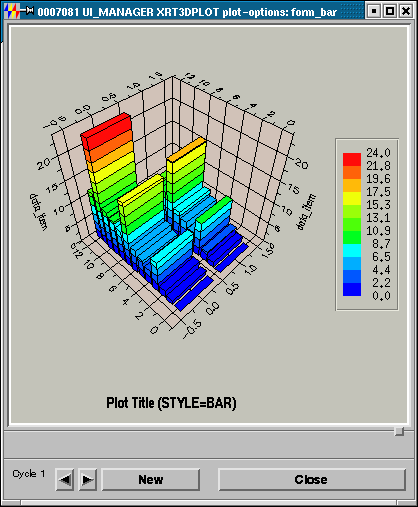
\includegraphics[width=0.8\linewidth]{plot3d-style_bar}
        \label{hc:plot3d_style_bar}
      \end{center}
    \end{minipage} \\[3ex]

    \begin{minipage}{0.45\linewidth}
      \begin{center}
        \index{PLOT3D@\PLOTTHREED!plot style example!surface}
        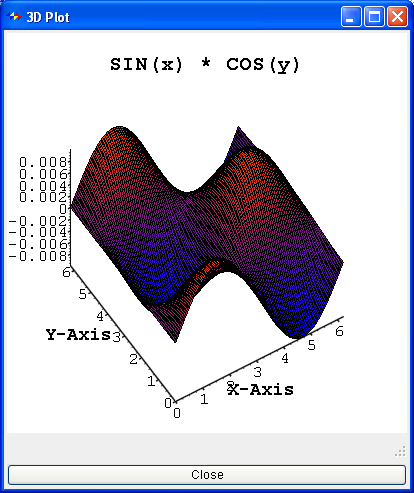
\includegraphics[width=0.8\linewidth]{3dplot-style_surface}
        \label{hc:plot3d_style_surface}
      \end{center}
    \end{minipage} \\[3ex]

    \begin{minipage}{0.45\linewidth}
      \begin{center}
        \index{PLOT3D@\PLOTTHREED!plot style example!contour}
        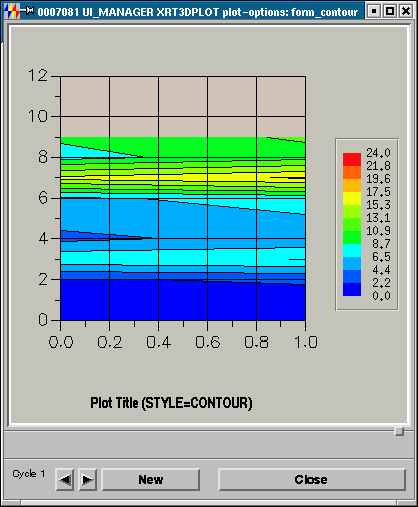
\includegraphics[width=0.8\linewidth]{plot3d-style_contour}
        \label{hc:plot3d_style_contour}
      \end{center}
    \end{minipage}
  \end{center}
  \caption{PLOT3D Plot styles}
\end{figure}
